\chapter{Sistemi biometrici basati su impronte digitali}

\section{Introduzione}

Le impronte digitali sono \textbf{creste e valli della pelle} sui palmi delle dita;
sono tratti biometrici \textbf{stabili} (dall'ottavo mese di gestazione) a meno di abrasioni
o malattie.

Durante la crescita, il dito cresce: la distanze si allargano ma le 
\textit{minutiae} rimangono le stesse.

\subsection{Sistema di classificazione attuale}

Le impronte si dividono, attraverso lo studio degli \textbf{orientamenti dei ridge} e \textbf{l'individuazione
di eventuali \textit{delta} o \textit{core}}, in:
\begin{itemize}
    \item \textbf{Arch:} \textit{entro da sinistra ed esco da destra; si divide in plain e tented}
    \item \textbf{Loop:} \textit{faccio un loop; si divide in left/right loop}
    \item \textbf{Whorl:} \textit{ci sono due delta attorno al cerchio}
\end{itemize}
Questa divisione torna utile per ottimizzare la ricerca di un'impronta; le denominazioni
nascono in base a come si muovono i ridge.

Le classi \textbf{non} sono distribuite uniformemente.

\begin{figure}[ht]
    \centering
    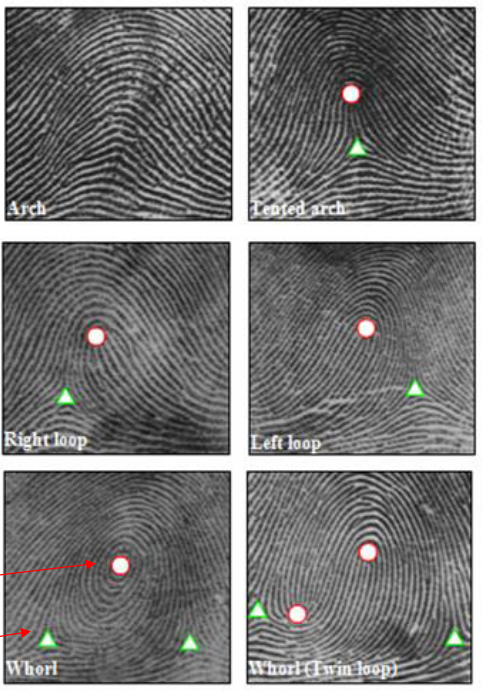
\includegraphics[width=0.6\linewidth]{images-chap5/classificazione.png}
    \caption{Classificazione delle impronte; in verde sono indicati i delta, in rosso i core}
\end{figure}

\subsection{Alcune applicazioni basate sulle impronte}

Esistono diversi tipo di sistemi:
\begin{itemize}
    \item sistemi integrati (smartphone)
    \item smartcard
    \item per PC
    \item stand alone
    \item distribuiti (AFIS)
\end{itemize}

Alcune tipologie di applicazioni sono:
\begin{itemize}
    \item \textbf{Forensi:}
    \begin{itemize}
        \item identificazione di corpi/persone/terroristi
        \item bambini scomparsi
        \item attività investigativa
    \end{itemize}
    \item  \textbf{Governative:}
    \begin{itemize}
        \item carte d'identità/passaporti/patenti
        \item controllo degli accessi
        \item controllo delle frontieri
        \item controllo documenti
    \end{itemize}
    \item \textbf{Commerciali:}
    \begin{itemize}
        \item ATM
        \item ecommerce
        \item accesso a servizi online
    \end{itemize}
\end{itemize}

\subsection{Sistemi AFIS}

AFIS (\textit{Automated Fingerprint Identification System}) è un sistema hardware e software
per:
\begin{itemize}
    \item acquisizione e classificazione
    \item ricerca di una impronta sconosciuta in una banca dati consultabile 
    dai terminali distribuiti
\end{itemize}
Tipicamente si usa per identificare un'impronta ignota.

Integrato significa che non c'è un unico server.


\subsection{Punti di forza e di debolezza}
\subsubsection{Punti di forza}

\begin{itemize}
    \item è una tecnologia matura, controllata e funzionante in molti ambienti
    \item l'acquisizione è facile
    \item offre la possibilità di usare più  dita
\end{itemize}

\subsubsection{Debolezze}

\begin{itemize}
    \item alcune impronte non possono essere acquisite (circa il 4\%)
    \item l'accuratezza tende a degradare nel tempo
    \item essendo associata ad applicazioni forensi, alcune persone provano disagio a fornire il tratto biometrico
\end{itemize}

\newpage
\subsection{I tre livelli di analisi delle impronte}

\subsubsection{Livello I (globale)}
A livello globale si osservano:
\begin{itemize}
    \item il flusso delle linee (arch, whorl, loop, \dots)
    \item i punti singolari (delta, core): questi punti descrivono ciò che c'è intorno
    \item la forma dell'impronta
    \item l'orientamento
    \item la frequenza delle righe 
\end{itemize}

\subsubsection{Livello II (locale)}

A livello locale è possibile identificare fino a 150 diverse \textbf{caratteristiche locali
delle minutiae}; \textit{zoomiamo} su ciò che accade intorno ad un ridge.

Le due principali caratteristiche sono le \textbf{biforcazioni} e \textbf{terminazioni}.
\begin{figure}[ht]
    \centering
    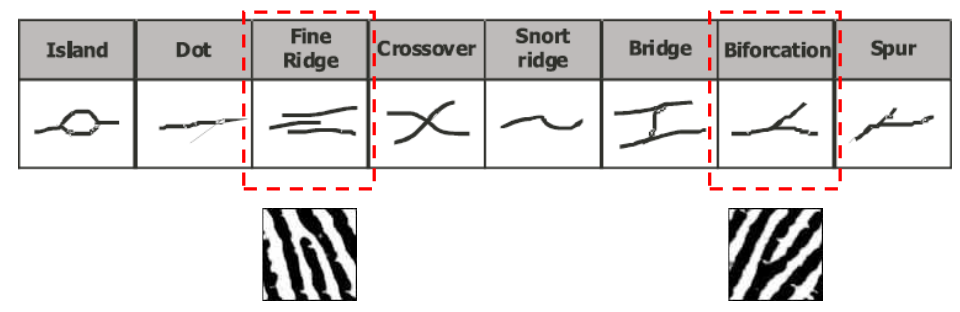
\includegraphics[width=0.75\linewidth]{images-chap5/caratteristiche.png}
\end{figure}

\subsubsection{Livello III (ultra-fine)}
A livello ultra-fine è possibile individuare i seguenti dettagli:
\begin{itemize}
    \item intra-creste (pori per la sudorazione)
    \item inter-creste ()
\end{itemize}

\begin{figure}[ht]
    \centering
    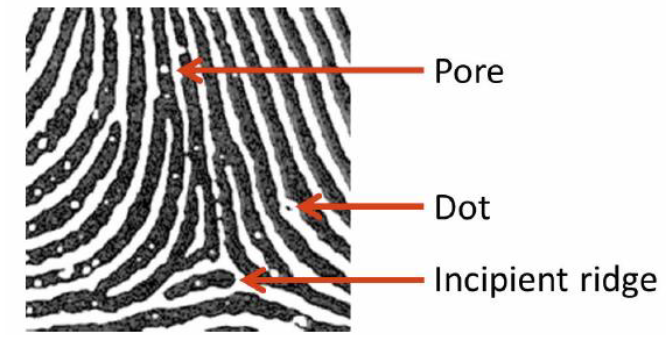
\includegraphics[width=0.5\linewidth]{images-chap5/livello3.png}
\end{figure}

I dettagli del livello III sono
considerati altamente distintivi,
ma si rilevano solo ad altissima
risoluzione (almeno 1000 dpi
ed in condizioni ideali).

Bastano pochi $mm^2$ per catturare molti dettagli di tutti e 3 i livelli.

\subsection{Quanto diverse?}

Le impronte possono avere una struttura simile ma hanno sempre tanti
punti di diversità.

Di solito si ha la seguente scala di diversità:
\begin{figure}[ht]
    \centering
    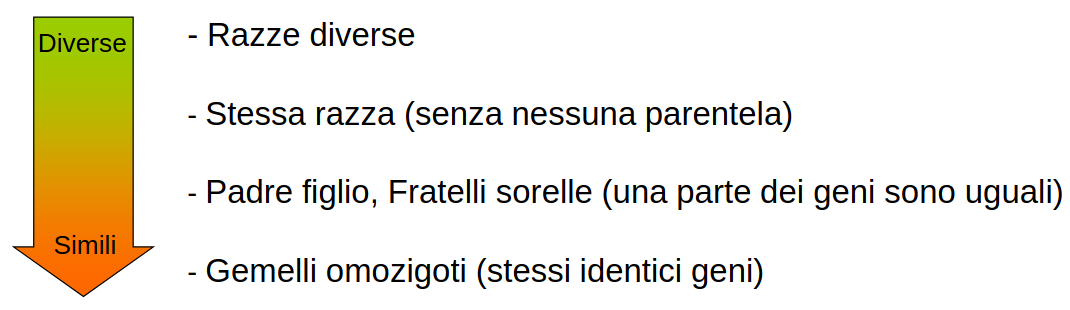
\includegraphics[width=1\linewidth]{images-chap5/diversita.png}
\end{figure}

\subsubsection{I gemelli?}

Anche i gemelli omozigoti (con lo stesso DNA) hanno impronte diverse.

Le impronte sono una manifestazione del \textit{fenotipo} (dipendente anche da fattori casuali ed 
ambientali) anche partendo dallo stesso \textit{genotipo}.

\subsubsection{Quante minuzie?}
Non c'è una regola mondiale accettata per stabilire se due impronte appartengono allo stesso
individuo.

Un esperto procede nel seguente modo, controllando:
\begin{enumerate}
    \item la concordanza del \textbf{pattern globale}
    \item la concordanza \textbf{qualitativa}, ovvero controlla che le minutiae siano identiche
    \item il fattore \textbf{quantitativo} che specifica il numero minimo di dettagli minuti che
    devono corrispondere tra le due impronte (ad esempio 12)
    \item la corrispondenza dei \textbf{dettagli di livello III}, che devono risultare identicamente correlati
\end{enumerate}

\subsection{Attuali criticità dei sistemi AFIS}

\begin{itemize}
    \item qualità acquisizione dell'impronta
    \item correttezza nella fase di estrazione delle minutiae e di matching; è necessario un supervisore
\end{itemize}

\section{Tipologie di sensori e caratteristiche}

I sensori devono cercare di catturare la distrbuzione di creste e valli sulla pelle;
maggiori sono i dettagli catturati, migliore sarà la capacità del sistema di 
identificare/verificare le persone.

\subsection{Modalità di acquisizione}
Esistono due principali modalità di acquisizione:
\begin{itemize}
    \item \textbf{off-line:} i polpastrelli vengono prima passati su un tampone inchiostrato e poi 
    vengono rotolati sulla carta; la scheda viene poi acquisita con uno scanner ottico.

    Un esempio sono le \textbf{impronte digitali latenti}, come quelle trovate su una scena del crimine
    \item \textbf{live-scan:} l'immagine dell'impronta digitale è acquisita in tempo reale 
    direttamente tramite il contatto con un apposito sensore
\end{itemize}

\subsubsection{Tipi di sensori live-scan}
\begin{itemize}
    \item \textbf{ottici:} scanner tradizionali
    \item \textbf{stato solido:} pixel sensibili alle variazioni di pressione e temperatura
    \item \textbf{altro tipo:} ultrasuoni
\end{itemize}

\subsection{Proprietà del sensore}

Nello scegliere un sensore bisogna controllare:
\begin{itemize}
    \item risoluzione
    \item area d'acquisizione
    \item numero di pixel e bit per pixel
    \item contrasto
    \item distorsione geometrica
\end{itemize}
Può essere utile controllare caratteristiche aggiuntive, come la presenza di componenti
hw/sw per il rilevamento automatico della presenza del dito e delle condizioni (posizione, pressione).

\newpage
\subsection{Sensori ottici}

\begin{figure}[ht]
    \centering
    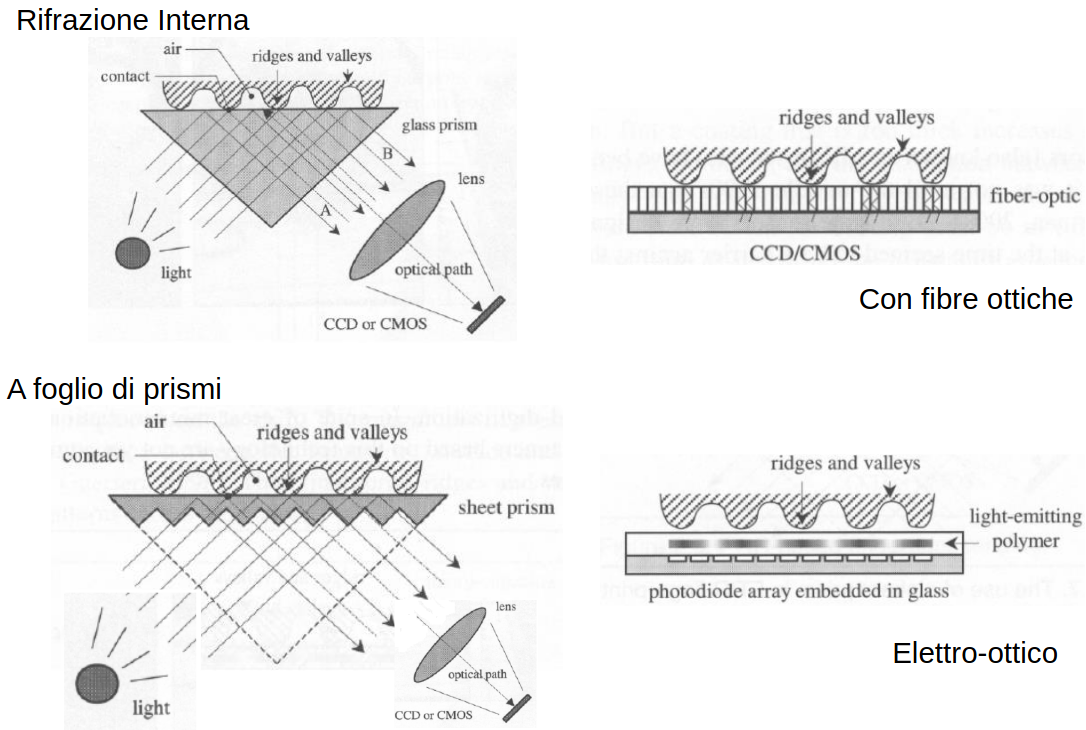
\includegraphics[width=1\linewidth]{images-chap5/ottici.png}
\end{figure}

Con la riflessione ottica si ottiene una risoluzione migliore.

\subsection{Sensori a stato solido}

Il contatto fra il ridge e la superficie del sensore cambia la capacità
del circuito del singolo pixel.

\begin{figure}[ht]
    \centering
    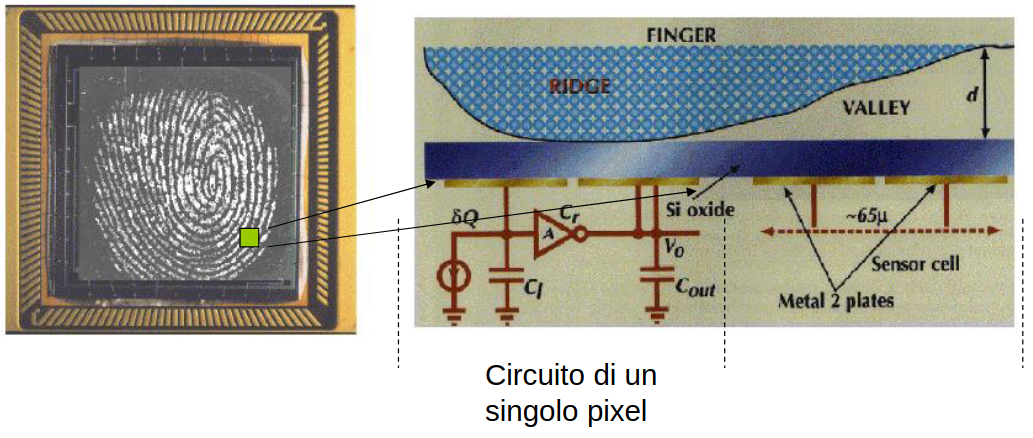
\includegraphics[width=1\linewidth]{images-chap5/statosolido.png}
\end{figure}

Ci sono due laminette metalliche che misurano una tensione diversa a seconda
della pressione; sotto ogni pixel c'è un circuito.
hanno forma simile ma circuiti dedicati diversi per il singolo pixel

\subsection{Sensori 3D (ultrasuoni)}

Sono dei sensori che riescono a rilevare la tridimensionalità dell'impronta digitale.
I sensori a stato solido che rilevano la temperatura o la pressione.

I sensori 3D sono utili nel fornire intrensicamente una funzione di anti-spoofing: 
sanno riconoscere se l'onda attraversa un \textit{medium} diverso da quello atteso (la pelle).

\subsection{Problemi di acquisizione: pressione}

All'aumentare della pressione, i ridge da discontinui iniziano a diventare continui e a vedersi
meglio; quando diventa troppa, i ridge iniziano ad unirsi.
\begin{figure}[ht]
    \centering
    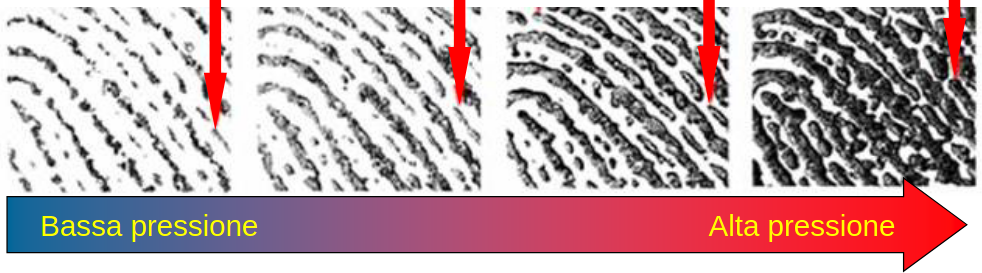
\includegraphics[width=0.75\linewidth]{images-chap5/pressione.png}
\end{figure}

\section{Rappresentazione, compressione,  e non unicità}

\subsection{Rappresentazione delle impronte}

La rappresentazione delle impronte in un sistema biometrico dipende da:
\begin{itemize}
    \item sensore impiegato (ottico, stato solido, \dots)
    \item livello di analisi (I, II, III)
    \item caratteristiche estratte (ridge, minuzie, \dots)
\end{itemize}

\subsubsection{Immagini delle impronte}

Il sample di un'impronta è una immagine in toni di grigio, quindi si
controlla la risoluzione e i bit per pixel.

\subsubsection{Formati di compressione}

\subsubsection{Formati di interscambio}


\subsection{Unicità delle impronte}

È possibile stimare la probabilità che due persone abbiano la stessa impronta.

Data un'impronta con $n$ minutiae, è possibile calcolare la probabilità di
condividere $q$ minutiae con un altro template contenente $m$ minutiae

$p(M, m, n, q)$ , con

$M= Area di overlap / Area di tolleranza = A/C$

\begin{figure}[ht]
    \centering
    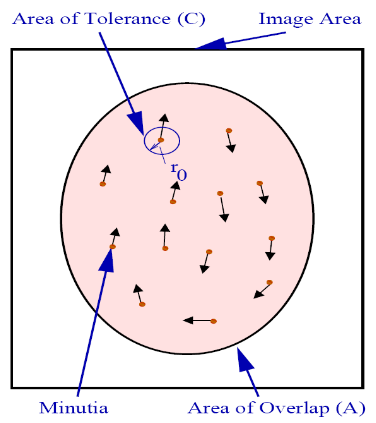
\includegraphics[width=0.5\linewidth]{images-chap5/unicita.png}
\end{figure}

\subsubsection{Esempio con parametri comuni}

$p(M,m,n,q) = p(70, 12, 12, 12) = 1,22 * 10^-20$

$M=70$ indica una stuazione tipica forense fra un intera ed una latent
paziale con almeno 12 minutiae “buone”.






